\PassOptionsToPackage{unicode}{hyperref}
\PassOptionsToPackage{hyphens}{url}
\PassOptionsToPackage{dvipsnames,svgnames,x11names}{xcolor}

\documentclass[12pt]{article}

\usepackage{paralist}
\usepackage{natbib}
\usepackage{hyperref}
\usepackage{booktabs}
\usepackage{subcaption}
\usepackage{lineno}
\usepackage[autostyle]{csquotes}
\usepackage{amsmath}
\usepackage{mathtools}
\usepackage{algorithm}
\usepackage{algorithmic}

\usepackage{amssymb}
\usepackage{stmaryrd} 
\usepackage{bm}
\usepackage{breqn}
\usepackage{enumitem}
\usepackage{amsmath, amssymb}
\usepackage{mathrsfs}
\usepackage{float}
\usepackage[font=footnotesize]{caption}
\usepackage{graphicx, wrapfig, rotating}
\usepackage{xr}
\usepackage{tikz}
\usetikzlibrary{positioning}
\usetikzlibrary{shapes, arrows, positioning}
\usepackage{adjustbox}
\usetikzlibrary{trees}
\usepackage[edges]{forest}
\newcommand{\circlewithcross}{\textcircled{$+$}}

\usepackage{amsmath,amssymb}
\usepackage{iftex}
\ifPDFTeX
  \usepackage[T1]{fontenc}
  \usepackage[utf8]{inputenc}
  \usepackage{textcomp}
\else 
  \usepackage{unicode-math}
  \defaultfontfeatures{Scale=MatchLowercase}
  \defaultfontfeatures[\rmfamily]{Ligatures=TeX,Scale=1}
\fi

\ifPDFTeX\else  
\fi
\IfFileExists{upquote.sty}{\usepackage{upquote}}{}
\IfFileExists{microtype.sty}{
  \usepackage[expansion=false]{microtype}
  \UseMicrotypeSet[protrusion]{basicmath}
}{}
\makeatletter
\@ifundefined{KOMAClassName}{
  \IfFileExists{parskip.sty}{
    \usepackage{parskip}
  }{
    \setlength{\parindent}{0pt}
    \setlength{\parskip}{6pt plus 2pt minus 1pt}}
}{
  \KOMAoptions{parskip=half}}
\makeatother
\usepackage{xcolor}
\setlength{\emergencystretch}{3em}
\setcounter{secnumdepth}{5}
\makeatletter
\ifx\paragraph\undefined\else
  \let\oldparagraph\paragraph
  \renewcommand{\paragraph}{
    \@ifstar
      \xxxParagraphStar
      \xxxParagraphNoStar
  }
  \newcommand{\xxxParagraphStar}[1]{\oldparagraph*{#1}\mbox{}}
  \newcommand{\xxxParagraphNoStar}[1]{\oldparagraph{#1}\mbox{}}
\fi
\ifx\subparagraph\undefined\else
  \let\oldsubparagraph\subparagraph
  \renewcommand{\subparagraph}{
    \@ifstar
      \xxxSubParagraphStar
      \xxxSubParagraphNoStar
  }
  \newcommand{\xxxSubParagraphStar}[1]{\oldsubparagraph*{#1}\mbox{}}
  \newcommand{\xxxSubParagraphNoStar}[1]{\oldsubparagraph{#1}\mbox{}}
\fi
\makeatother

\providecommand{\tightlist}{
  \setlength{\itemsep}{0pt}\setlength{\parskip}{0pt}}\usepackage{longtable,booktabs,array}
\usepackage{calc}
\usepackage{etoolbox}
\makeatletter
\patchcmd\longtable{\par}{\if@noskipsec\mbox{}\fi\par}{}{}
\makeatother
\IfFileExists{footnotehyper.sty}{\usepackage{footnotehyper}}{\usepackage{footnote}}
\makesavenoteenv{longtable}
\usepackage{graphicx}
\makeatletter
\def\maxwidth{\ifdim\Gin@nat@width>\linewidth\linewidth\else\Gin@nat@width\fi}
\def\maxheight{\ifdim\Gin@nat@height>\textheight\textheight\else\Gin@nat@height\fi}
\makeatother
\setkeys{Gin}{width=\maxwidth,height=\maxheight,keepaspectratio}
\makeatletter
\def\fps@figure{htbp}
\makeatother

\addtolength{\oddsidemargin}{-.5in}
\addtolength{\evensidemargin}{-.1in}
\addtolength{\textwidth}{1in}
\addtolength{\textheight}{1.7in}
\addtolength{\topmargin}{-1in}
\makeatletter
\@ifpackageloaded{caption}{}{\usepackage{caption}}
\AtBeginDocument{
\ifdefined\contentsname
  \renewcommand*\contentsname{Table of contents}
\else
  \newcommand\contentsname{Table of contents}
\fi
\ifdefined\listfigurename
  \renewcommand*\listfigurename{List of Figures}
\else
  \newcommand\listfigurename{List of Figures}
\fi
\ifdefined\listtablename
  \renewcommand*\listtablename{List of Tables}
\else
  \newcommand\listtablename{List of Tables}
\fi
\ifdefined\figurename
  \renewcommand*\figurename{Figure}
\else
  \newcommand\figurename{Figure}
\fi
\ifdefined\tablename
  \renewcommand*\tablename{Table}
\else
  \newcommand\tablename{Table}
\fi
}
\@ifpackageloaded{float}{}{\usepackage{float}}
\floatstyle{ruled}
\@ifundefined{c@chapter}{\newfloat{codelisting}{h}{lop}}{\newfloat{codelisting}{h}{lop}[chapter]}
\floatname{codelisting}{Listing}
\newcommand*\listoflistings{\listof{codelisting}{List of Listings}}
\newcommand{\Andrea}[1]{\textcolor{red}{#1}}
\makeatother
\makeatletter
\makeatother
\makeatletter
\@ifpackageloaded{caption}{}{\usepackage{caption}}
\@ifpackageloaded{subcaption}{}{\usepackage{subcaption}}
\makeatother

\ifLuaTeX
  \usepackage{selnolig}
\fi
\usepackage[]{natbib}
\bibliographystyle{agsm}
\usepackage{bookmark}

\IfFileExists{xurl.sty}{\usepackage{xurl}}{}
\urlstyle{same}
\hypersetup{
  pdftitle={Improving Discrepancy Measures for Global Sensitivity Analysis},
  pdfauthor={Alessio Lachi; Samuele Lo Piano; Razi Sheikholeslami; Arnald Puy; Pamphile Tupui Roy; Andrea Saltelli},
  pdfkeywords={Ersatz discrepancy measure, Total-order index, Global sensitivity analysis, Uncertainty analysis, Modeling},
  colorlinks=true,
  linkcolor={blue},
  filecolor={Maroon},
  citecolor={Blue},
  urlcolor={Blue},
  pdfcreator={LaTeX via pandoc}}

\newcommand{\anon}{1}

\begin{document}

\def\spacingset#1{\renewcommand{\baselinestretch}
{#1}\small\normalsize} \spacingset{1}

\if1\anon
{
  \title{\bf Improving Discrepancy Measures for Global Sensitivity Analysis}
  \author{
    \textbf{Samuele Lo Piano} \\
    a) Faculty of Management and Economics,\\ Gdańsk University of Technology,\\ Gdańsk (Poland)\\
    b) Barcelona School of Management,\\ Pompeu Fabra University,\\ Barcelona (Catalonia)\\
    \textbf{Alessio Lachi}\thanks{Corresponding author} \\
    Departmental Faculty of Medicine,\\ Saint Camillus International University of Health and Medical Sciences,\\ Rome (Italy) \\    
    \textbf{Razi Sheikholeslami} \\
    Department of Civil Engineering,\\ Sharif University of Technology,\\ Tehran (Iran)\\
    \textbf{Arnald Puy} \\
    School of Geography, Earth and Environmental Sciences,\\ University of Birmingham,\\ Birmingham (United Kingdom)\\
    \textbf{Pamphile Tupui Roy} \\
    Consulting Manao,\\ Vienna (Austria)\\
    \textbf{Andrea Saltelli} \\
    a) Barcelona School of Management,\\ Pompeu Fabra University,\\ Barcelona (Catalonia)\\
    b) Centre for the Study of the Sciences and the Humanities,\\ University of Bergen,\\ Bergen (Norway)
    }
  \maketitle
} \fi

\if0\anon
{
  \bigskip
  \bigskip
  \bigskip
  \begin{center}
    {\LARGE\bf Improving Discrepancy Measures for Global Sensitivity Analysis}
\end{center}
  \medskip
} \fi

\bigskip
\begin{abstract}
Global Sensitivity Analysis (GSA) is a fundamental tool used to quantify the impact of uncertainty in model inputs on outputs, facilitating model simplification, assumption testing, and informed decision-making. Among various GSA methods, variance-based techniques, such as those relying on Sobol' indices, are widely employed due to their strong statistical foundations and interpretability. \citet{puy2024discrepancy} recently proposed an intuitive and computationally efficient \textit{ersatz} discrepancy measure that quantifies deviations from uniformity in the input--output space to identify influential inputs, without requiring the multidimensional integrals of Sobol' indices or the ANOVA decomposition underlying variance-based measures. Building on this concept, the present work makes four contributions. First, we introduce an \textit{adjusted} ersatz discrepancy that rank-transforms the output before gridding and imputes isolated empty cells via a Moore-neighbourhood rule, substantially improving agreement with the total-order sensitivity index $T_i$. Second, we provide the first theoretical account of why this measure tracks $T_i$, grounded in copula theory: the adjusted ersatz is shown to be a consistent screening statistic for the support of the copula of $(x_i,\bm Y)$, with a proven zero condition, an explicit full-support ceiling that bounds its use as a magnitude estimator. Third, we benchmark the adjusted ersatz against three additional total-order estimators that exploit the same input--output sample at no extra computational cost -- polynomial chaos expansion (PCE), Shapley effects derived from the same PCE fit, and a PAWN-type maximum Kolmogorov--Smirnov screening index -- across seven benchmark functions, including a large-scale \textit{Becker metafunction} stress test, and a real-world hydrological model (HYMOD). Fourth, departing from one-at-a-time perturbation, we conduct a joint, Sobol'-design \textit{sensitivity analysis of the sensitivity analysis method itself}, varying five algorithmic parameters (grid resolution, imputation threshold, screening threshold, and the comparator methods' own tuning parameters) simultaneously to identify which design choices actually drive performance. The adjusted ersatz is found to be the most reliable screening tool for non-smooth, discrete, or interaction-dominated outputs where polynomial-based estimators are misspecified, while remaining an order of magnitude cheaper than Monte Carlo Sobol' estimators.
\end{abstract}

\noindent
{\it Keywords:} Ersatz discrepancy measure, Sobol' total-order index, Global sensitivity analysis, Copula, Uncertainty analysis
\vfill

\newpage
\spacingset{1.8}

\section{Introduction}

Global Sensitivity Analysis (GSA) investigates how variations in all uncertain model inputs, considered simultaneously across their full range, influence model outputs. This approach supports modelers in understanding the role of underlying assumptions, detecting key driving factors, simplifying complex models, and enhancing decision-making processes based on model results \citep{Saltelli2008}.

Over the past three decades, a wide range of GSA techniques have been developed, providing modelers with extensive guidance on selecting appropriate methods for different sensitivity analysis contexts \citep{becker_metafunctions_2020, puy_comprehensive_2022, razavi2021future, sheikholeslami2021viscous}. Among the most commonly used approaches are variance-based methods, which break down the output variance of a model with $k$ inputs into contributions from individual factors, pairs, triplets, and higher-order interactions up to the $k$-th term. These contributions are measured through indices of Sobol' calculated for a specific input $i$: the first-order sensitivity index ($S_i$) captures the primary effect of each input, while the total-order sensitivity index ($T_i$) accounts for both its direct effect and all possible interactions with other variables \citep{homma1996importance}. Variance-based techniques are grounded in solid statistical principles (ANOVA decomposition) and are particularly useful for identifying unimportant factors that can be fixed to simplify the model or for ranking inputs according to their influence on output uncertainty \citep{Saltelli2008}. $T_i$ is generally computed via Monte Carlo (MC) integrals using estimators such as that of \citet{jansen1999}, reviewed and compared in \citet{saltelli_variance_2010}, or via emulator-based approaches such as polynomial chaos expansion \citep{sudret_global_2008} or machine learning \citep{antoniadis2021random}. A related but distinct family of variance-based importance measures, the Shapley effects, allocate the total output variance among inputs using the cooperative game-theoretic Shapley value; they satisfy an efficiency property absent from $T_i$ (the Shapley effects of all inputs sum exactly to the total output variance) and are bracketed between the first- and total-order indices, $S_i \le \mathrm{Sh}_i \le T_i$ \citep{owen2014}.

\citet{puy2024discrepancy} shows that certain discrepancy algorithms computed in the two-dimensional plane $[x_i,\bm{Y}]$, where $x_i$ is the $i$-th model input and $\bm{Y}$ is the model output, effectively replicate the behavior of $T_i$. Since discrepancy algorithms are themselves computer-time intensive, the authors introduce a simple \textit{S-ersatz} discrepancy measure that approximates the performance of the most effective discrepancy algorithms at a fraction of the cost. \citet{puy2024discrepancy} is therefore the origin of the underlying ersatz concept benchmarked throughout this paper; the \textit{adjusted} ersatz discrepancy, its theoretical justification, and its comparison against polynomial-chaos-derived estimators are the contribution of the present work.

The present contribution introduces an adjustment to the algorithm of \citet{puy2024discrepancy} -- a rank transformation of the output prior to gridding, combined with a deterministic imputation of isolated empty cells -- which together raise the correlation ($\rho$) between the Savage-score rankings produced by $T_i$ and by the ersatz approximation, while also lowering the Mean Absolute Error (MAE) between the two. We then address three further questions that the original ersatz proposal left open: (i) why does rank-transformation plus imputation improve agreement with $T_i$, which we resolve through a copula-theoretic argument (\S\ref{theory}, with a full proof provided as supplementary material); (ii) how does the adjusted ersatz compare, at identical sample cost, against other total-order estimators that exploit the same input--output pairs -- polynomial chaos expansion, PCE-derived Shapley effects, and a PAWN-type screening index; and (iii) which algorithmic choices actually matter, which we answer with a joint, Sobol'-design sensitivity analysis of the sensitivity analysis method itself, departing from the one-at-a-time perturbation of individual algorithmic choices used in earlier explorations of this question.

In addition to improving the accuracy and robustness of the ersatz discrepancy measure, the proposed refinements also contribute to a better balance between type I ($\alpha$) and type II ($\beta$) errors. The type I error $\alpha$ represents the probability of incorrectly classifying an unimportant input as important, whereas the type II error $\beta$ corresponds to the probability of failing to identify an important input as such. Because the dividing line between ``important'' and ``unimportant'' is itself a modelling choice, we report $\alpha$ and $\beta$ at three canonical screening thresholds, $T_i \in \{0.01, 0.05, 0.10\}$, spanning conservative to liberal screening criteria, rather than a single threshold.

To assess the validity of the proposed improvements, we first compare the adjusted ersatz, the original S-ersatz, PCE-derived $T_i$ and Shapley effects, and a PAWN-type screening index against the reference $T_i$ across seven benchmark functions of varying dimensionality, smoothness, and interaction structure, drawn from the \href{https://cran.r-project.org/web/packages/sensobol/index.html}{\texttt{sensobol}} library and from \citet{saltelli2025}. We then stress-test all five estimators using the Becker metafunction approach \citep{becker_metafunctions_2020, puy_comprehensive_2022}, which generates a large ensemble of functions with diverse input distributions and interaction structures, and apply a joint sensitivity analysis to the algorithmic parameters of the screening methods themselves. Finally, we evaluate all estimators on the HYMOD hydrological model \citep{sheikholeslami2017progressive, vrugt2003shuffled}, a real-world case with a bounded, left-skewed, non-smooth output.

\section{Methods}

Before introducing the concept of discrepancy, it is useful to first clarify the role of scatter plots in GSA. Owing to their intuitive nature, scatter plots are commonly employed in GSA as a preliminary means of exploring input sensitivities prior to engaging in more quantitative analyses (Figure ~\ref{fig:scatter}).

\begin{figure}[H]
    \centering
    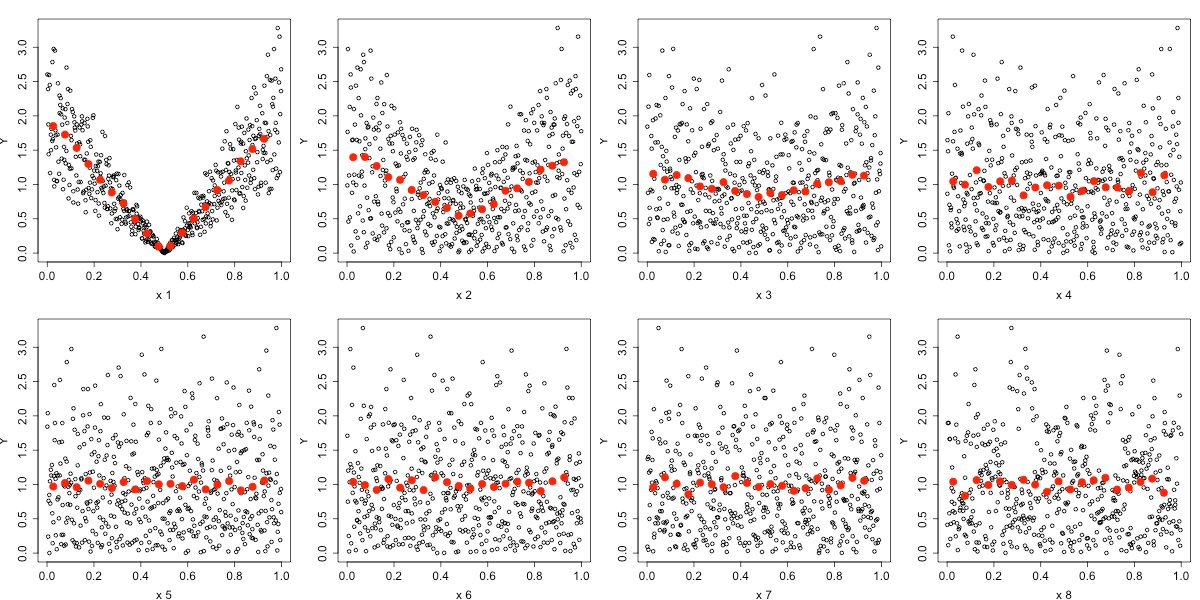
\includegraphics[width=6in,height=\textheight]{ris/scatterplot.png}
    \caption{Scatter-plot of the \cite{sobol1998quasi} function with a sample size of $2^9$. It can be observed that the output $\bm{Y}$ is primarily driven by input variable $x_1$, with importance gradually decreasing across variables $x_2, x_3, \ldots$. Red points represent the expected value of the model output given the value on the x-axis.}
    \label{fig:scatter}
\end{figure}

Let us define $\bm\Omega=[0,1)^d$ as a $d$-dimensional unit hypercube containing $N_s$ sampling points produced via the \cite{sobol1998quasi} quasi-random sequence and represented by the following matrix:

\begin{equation*}
    \bm X=
    \begin{bmatrix}
        x_1^{(1)}   & x_2^{(1)}   & \cdots    & x_d^{(1)}   \\
        x_1^{(2)}   & x_2^{(2)}   & \cdots    & x_d^{(2)}   \\
        \vdots      & \vdots      & x_k^{(i)} & \vdots      \\
        x_1^{(N_s)} & x_2^{(N_s)} & \cdots    & x_d^{(N_s)}
    \end{bmatrix},
\end{equation*}

where $x_k^{(i)}$ is the value taken by the $k$-th input in the $i$-th row.

The vector of model outputs produced by a general function $f(\mathbf{X})$, which takes the values of matrix $\mathbf{X}$ as input, is defined by the following vector:

\begin{equation*}
    \bm{Y}=
    \begin{bmatrix}
        y^{(1)}   \\
        y^{(2)}   \\
        \vdots    \\
        y^{(N_s)}
    \end{bmatrix}
    =
    \begin{bmatrix}
        f(x^{(1)})   \\
        f(x^{(2)})   \\
        \vdots       \\
        f(x^{(N_s)})
    \end{bmatrix}.
\end{equation*}

If $\bm{Y}$ is sensitive to changes in $x_k$, a scatter-plot of $\bm{Y}$ against $x_k$ will display a trend or shape. Generally, the sharper the trend/shape, the larger the area without points and the stronger the influence of $x_k$ on $\bm{Y}$.

In a previous work, \citet{puy2024discrepancy} developed an ersatz discrepancy measure, referred to as S-ersatz, which aims to approximate the ranking of $T_i$. To achieve this, for each input variable $i$, the authors proposed partitioning the plane $M^{(i)}_k = [x^{(i)}_k, \bm{Y}]$ into a uniform grid composed of squared cells, ideally such that each cell contains exactly one sample point. Quasi-random sequences provide the best chance of attaining this theoretical filling. However, since their sample sizes are powers of two, the total number of samples $N_s$ must be adjusted to $\lceil\sqrt{N_s}\rceil \times \lceil\sqrt{N_s}\rceil$, where $\lceil \cdot \rceil$ denotes the ceiling function (e.g., while $N_s=16$ does not need adjustment, $N_s=32$ becomes 36). The ersatz measure is then computed as the ratio between the number of occupied cells ($N_p$) and the total number of cells ($N_T$). To define a measure that accounts for the presence of points, we compute $S_{ersatz}=1-\frac{N_p}{N_T}$.

For a better understanding of the measure, consider the following $4 \times 4$ matrix:

\begin{equation*}
    M^{(i)}_k =
    \begin{bmatrix}
        \bullet  & \circ   & \bullet & \bullet \\
        \bullet  & \bullet & \bullet & \circ   \\
        \circ    & \bullet & \circ   & \circ   \\
        \circ    & \circ   & \circ   & \circ
    \end{bmatrix},
\end{equation*}

where $\bullet$ and $\circ$ denotes the presence or absence of a point in the matrix, respectively. In this example, $N_s = 14$ and $N_T = 4$. Therefore, $S_{ersatz} = 1 - \frac{7}{16} = 0.5625$.

Note that the use of quasi-random numbers gives the best chances that each cell will contain close to one point if $x_k$ does not influence $\bm{Y}$ \citep{Kucherenko2015}. A valid alternative to quasi-random numbers, used in \cite{puy2024discrepancy}, is the scrambled quasi-random number proposed by \cite{owen1995randomly}. As illustrated by \cite{kucherenko2023importance}, the scrambled quasi-random number method exhibits superior performance compared to standard quasi-random numbers. Therefore, in this work, we adopted this approach throughout, and confirm in \S\ref{BeckerSA} that the choice between quasi-random and pseudo-random sampling has a negligible effect on the adjusted ersatz's performance relative to its other algorithmic parameters.

Let us now define $N_x$ and $N_y$ as the number of cells along the x and y axes of the grid, and $n_k^{(i)}$ as the number of points in the cell at the intersection of the $i$-th row and the $k$-th column. Based on the properties of a uniform grid, we can also write that $N_x=N_y=\lceil\sqrt{N_s}\rceil$ and $N_T=N_xN_y$. For a specific input $i$, we obtain that:

\begin{equation*}
    S_{ersatz}=\frac{\sum\limits_i^{N_x}\sum\limits_k^{N_y}\bm{I}[n_k^{(i)}>0]}{N_xN_y},
\end{equation*}

where $\bm{I}$ is the indicator function which evaluates to 1 if the condition inside the parentheses is true and 0 otherwise.

As discussed in \citet{puy2024discrepancy}, $S_{ersatz}$ provides a ranking of the most influential inputs. With the proposed adjustments, presented next, our objective is to ensure that the new discrepancy measure is as close as possible to $T_i$, and to make the conditions under which this approximation holds mathematically explicit.

\subsection{First modification -- Making the model output uniform}
\label{1st}

Let us observe the following figure. In \cite{puy2024discrepancy}, even for an unimportant variable, the distribution was uniform over $x_k^{(i)}$ but not over $\bm{Y}$, i.e., one can see areas without points in the upper part of the diagram. Even if $\bm{Y}$ is not influenced by $x_k$, the non-uniform distribution of $\bm{Y}$ can still create apparent gaps as illustrated in Figure \ref{fig:scatter2}.

\begin{figure}[H]
    \centering
    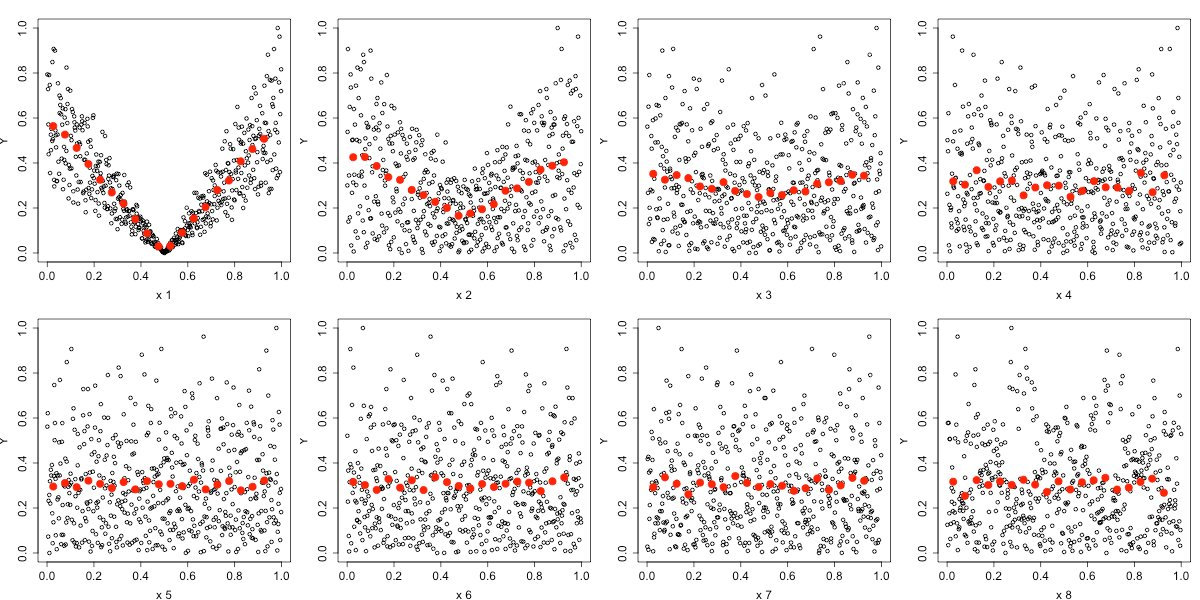
\includegraphics[width=6in,height=\textheight]{ris/scatterplot2.png}
    \caption{Scatter-plot of the \cite{sobol1998quasi} function with a sample size of $2^9$ and normalized $\bm{Y}$. It can be observed that the output $\bm{Y}$ is primarily driven by input variable $x_1$, with importance gradually decreasing across variables $x_2, x_3, \ldots$. Red points represent the expected value of the model output given the value on the x-axis.}
    \label{fig:scatter2}
\end{figure}

This issue can be easily corrected by transforming $\bm{Y}$ into a uniform variable through a rank-based transformation where $\bm{Y'}=\frac{rank(\bm{Y})-1}{N_s}$. Note that the subtraction of 1 ensures that the ranking starts from 0 rather than 1, so that the transformed $\bm{Y'}$ spans the interval $[0,1)$ instead of $[\frac{1}{N_s}, 1]$. As shown in Figure \ref{fig:scatter3}, this adjustment ensures a uniform mapping of the function compared to the previous scatterplot. As we formalise in \S\ref{theory}, this step is what converts the raw $[x_i, \bm{Y}]$ scatter into a sample from the \emph{empirical copula} of $(x_i, \bm{Y})$, removing the confounding effect of $\bm{Y}$'s marginal distribution and exposing only the dependence structure between $x_i$ and $\bm{Y}$.

\begin{figure}[H]
    \centering
    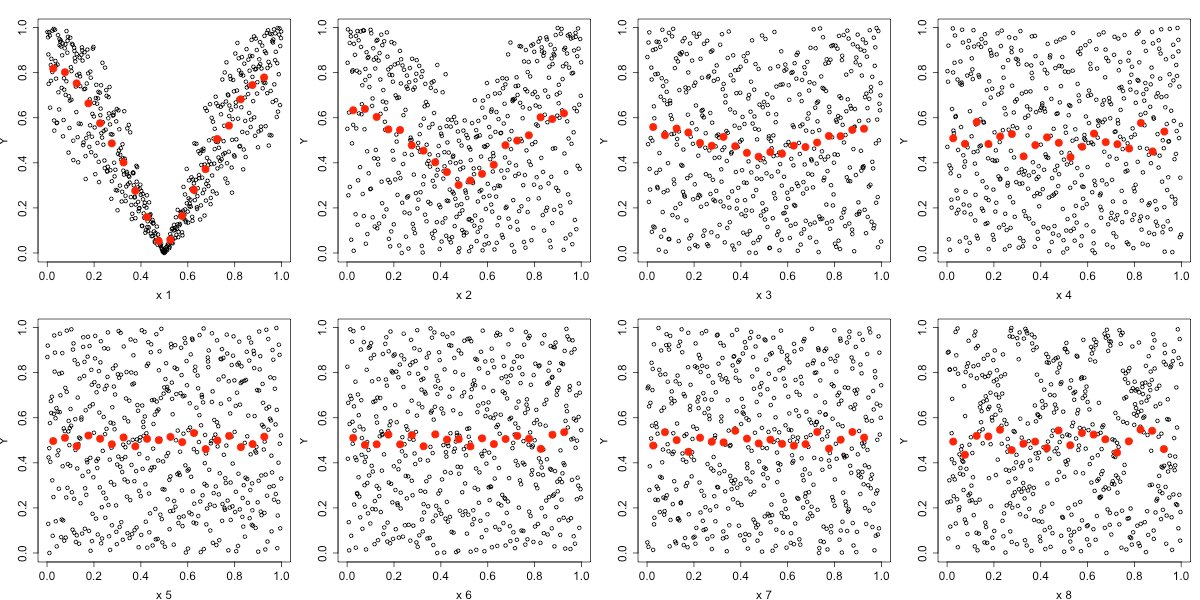
\includegraphics[width=6in,height=\textheight]{ris/scatterplot3.png}
    \caption{Scatter-plot of the \cite{sobol1998quasi} function with uniform $\bm{Y}$. The output $\bm{Y}$ is primarily driven by input variable $x_1$, with importance gradually decreasing across variables $x_2, x_3, \ldots$. Red points represent the expected value of the model output given the value on the x-axis. Even after this adjustment, variable $x_8$ retains a visibly non-uniform pattern relative to $x_5$--$x_7$; \S\ref{theory} shows this is expected whenever the input's dependence with the output is mediated by higher-order interactions rather than a marginal effect.}
    \label{fig:scatter3}
\end{figure}

If we denote the uniform grid plane by ${M'}^{(i)}_k=[x^{(i)}_k,\bm{Y'}]$, we obtain the matrix required for the ersatz calculation, as shown in Figure \ref{fig:scatter4}.

\begin{figure}[H]
    \centering
    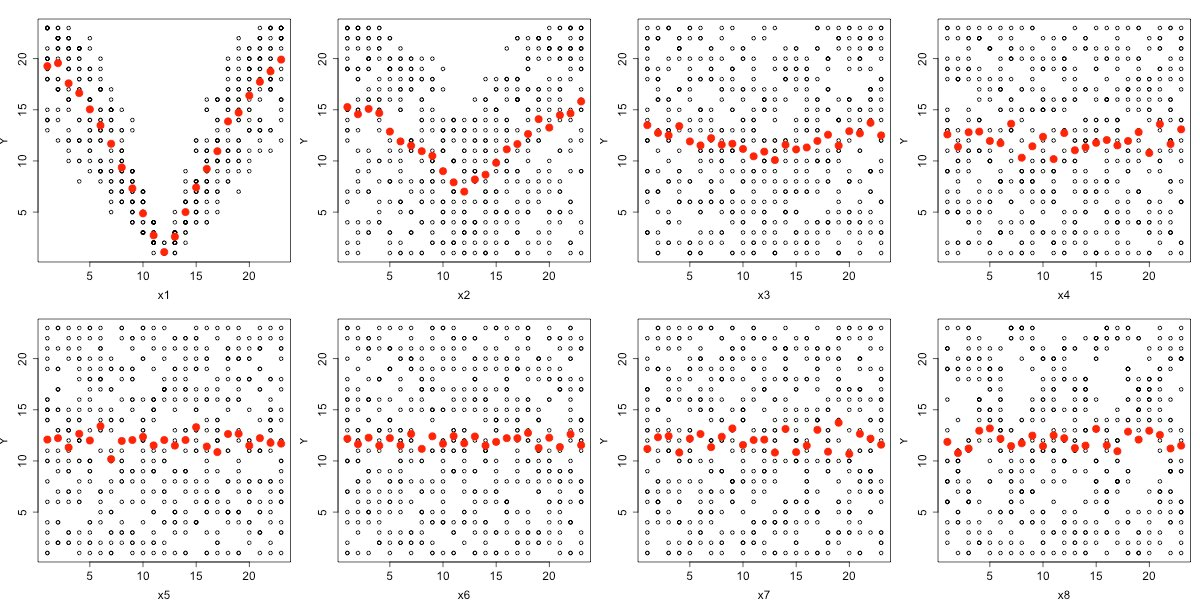
\includegraphics[width=6in,height=\textheight]{ris/scatterplot4.png}
    \caption{Uniform grid plane for the \cite{sobol1998quasi} function with a sample size of $2^9$. The output $\bm{Y}$ is primarily driven by input variable $x_1$, with importance gradually decreasing across variables $x_2, x_3, \ldots$. Red points represent the expected value of the model output given the value on the x-axis.}
    \label{fig:scatter4}
\end{figure}

\subsection{Second modification -- Imputation of the discrepancy matrix}
\label{2nd}

As illustrated in Figure \ref{fig:scatter4}, an empty cell may either genuinely represent the absence of points or be the consequence of insufficient sampling, thus leading to an imputation problem. To address this issue, we propose a deterministic imputation strategy aimed at correcting the plane ${M'}^{(i)}_k$, conceptually related to cellular automata update rules such as Conway's Game of Life \citep{gardner_mathematical_1970}.

For each empty cell in ${M'}^{(i)}_k$, we compute the proportion of non-empty neighboring cells. The number of neighbors can be at most $8$, as cells sharing only one corner are also considered. Imputation is performed only when at least $50\%$ of the neighboring cells are non-empty.

The choice of the $50\%$ threshold is not arbitrary: in \S\ref{theory} we show analytically that this value is calibrated to correctly classify both limiting cases -- under statistical independence between $x_i$ and $\bm Y$, the threshold leaves the (already near-complete) grid unchanged, while under a perfectly monotone dependence it does not trigger any spurious filling, so that the adjusted ersatz correctly tends to $0$ and $1$ at the two extremes, respectively. Whether a different threshold could improve performance at intermediate dependence strengths is an empirical question we address directly in \S\ref{BeckerSA}, where the imputation threshold, together with four other algorithmic parameters of the screening methods compared in this paper, is varied jointly (rather than one at a time) in a dedicated sensitivity analysis of the sensitivity analysis method.

In such cases, the empty cell is assigned the value $1$; otherwise, the cell remains empty. As illustrated in Figure \ref{fig:scatter5}, this strategy aims to preserve potential spatial structures in regions affected by missing data, while ensuring that the information contained in non-empty cells continues to contribute to the information captured by $T_i$. The method is particularly relevant under both homogeneous and highly heterogeneous spatial distributions.

\begin{figure}[H]
    \centering
    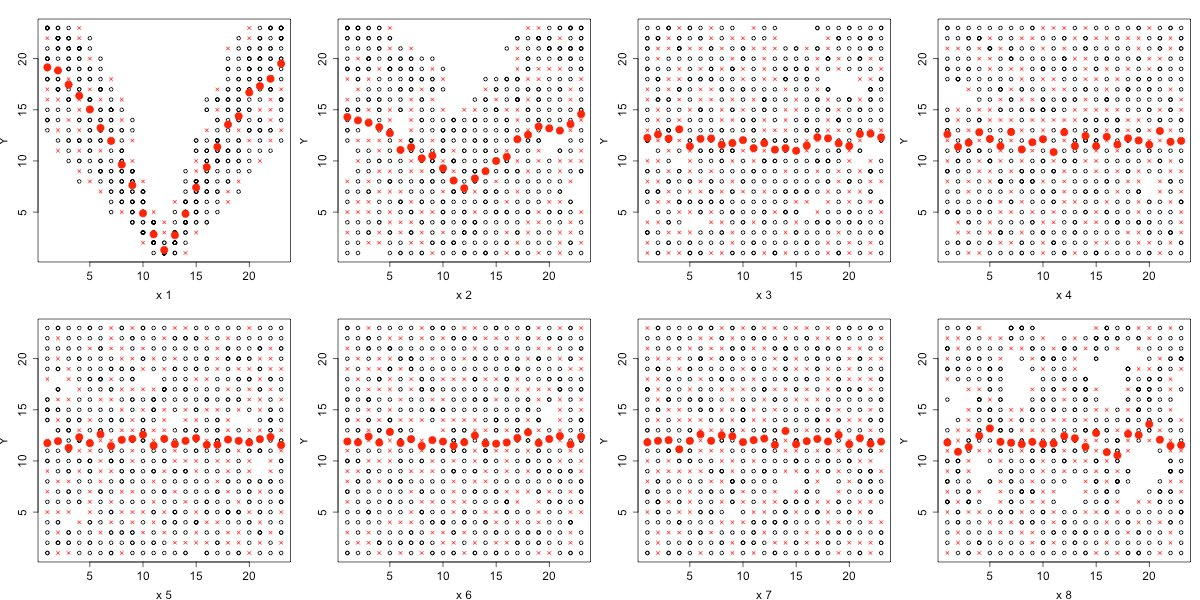
\includegraphics[width=6in,height=\textheight]{ris/scatterplot5.png}
    \caption{Imputed uniform grid plane for the \cite{sobol1998quasi} function with a sample size of $2^9$. Black points represent the observations before imputation, whereas red crosses represent the observations after imputation. The output $\bm{Y}$ is primarily driven by input variable $x_1$, with importance gradually decreasing across variables $x_2, x_3, \ldots$. Even with the adjustment, residual holes remain visible for $x_8$ -- a finite-sample manifestation of the ``full-support ceiling'' formalised in \S\ref{theory}, rather than an implementation artefact.}
    \label{fig:scatter5}
\end{figure}

Let us denote by ${M''}^{(i)}_k$ the imputed uniform grid plane. As we will see in the next section, if we compute $S_{ersatz}$ on ${M''}^{(i)}_k$, we obtain a more accurate estimate of the ersatz measure, which we will call $S^{adjusted}_{ersatz}$.

\subsection{Why the adjustment works: a copula-theoretic account}
\label{theory}

The two modifications above were originally motivated by visual inspection of scatterplots. We now provide a formal explanation for why they improve agreement with $T_i$, with the full derivation, proofs, and an explicit counterexample given as supplementary material (\textit{Mathematical Foundation of the Adjusted Ersatz Discrepancy}, hereafter the Proof).

The key step is recognising that the rank transformation of \S\ref{1st} converts the sample $\{(x_i^{(j)}, \bm Y^{(j)})\}_{j=1}^{N_s}$ into a draw from the \emph{empirical copula} of $(x_i, \bm Y)$ \citep{deheuvels1979}, which converges uniformly to the true copula $C_i$ as $N_s \to \infty$ \citep{fermanian2004}, by Sklar's theorem \citep{sklar1959}. The $s \times s$ grid of \S\ref{1st}--\S\ref{2nd} is then a histogram of this empirical copula, and the adjusted ersatz measures how far the occupied cells deviate from full coverage of $[0,1]^2$. The Proof establishes four results from this starting point.

First, a \emph{zero condition}: if $T_i = 0$ (i.e.\ $x_i \perp \bm Y$ under mutually independent inputs), then $S^{adjusted}_{ersatz} \xrightarrow{P} 0$ as $N_s \to \infty$, because the independence copula $\Pi(u,v)=uv$ uniquely maximises the expected grid coverage among all copulas (a consequence of Jensen's inequality applied to the strictly concave cell-occupation probability). This direction is sufficient but not necessary: \S\ref{theory} documents an explicit counterexample, the additive-modular function $\bm Y = (x_i + x_k) \bmod 1$, for which $T_i = 1$ yet the marginal copula of $(x_i, \bm Y)$ is exactly the independence copula, so the adjusted ersatz (and, more generally, any sensitivity measure based on the bivariate copula of a single input against the output) returns $0$. This is a structural limitation of bivariate screening, not specific to the ersatz, and motivates a natural extension to trivariate projections $(x_i, x_k, \bm Y)$ that we flag as future work.

Second, a \emph{monotone-direction} property: under inputs $i, k$ whose copulas $C_i, C_k$ belong to a family ordered by concordance (e.g.\ Gaussian, Clayton, Gumbel, or Frank), $T_i > T_k$ implies $\mathbb{E}[S^{adjusted}_{ersatz}(i)] \ge \mathbb{E}[S^{adjusted}_{ersatz}(k)]$ for sufficiently large $N_s$. This condition is satisfied by the great majority of dependence structures encountered in practice, and is consistent with the high Savage-score correlations reported across the benchmark functions below, but it is not universal.

Third, an explicit \emph{full-support ceiling}: for any copula with full support on $[0,1]^2$ (e.g.\ a Gaussian copula with $|\rho|<1$), $\mathbb{E}[S^{adjusted}_{ersatz}(i)] \to 0$ as $N_s \to \infty$, \emph{regardless of the magnitude of $T_i$}. The adjusted ersatz is therefore a consistent indicator of \emph{whether} $x_i$ matters, at moderate $N_s$, but not a consistent estimator of \emph{how much} it matters; the latter requires a singular (functionally deterministic) copula, attained only when $\bm Y$ is a strictly monotone function of $x_i$ alone. This is the theoretical counterpart to the empirically observed MAE plateau reported for HYMOD in \S\ref{HYMOD}.

Fourth, the imputation step of \S\ref{2nd} is shown to be the mechanism that extends sensitivity from the first-order index $S_i$ towards the total-order index $T_i$: when $S_i = 0$ but $T_i > 0$ (a pure interaction effect), the copula of $(x_i, \bm Y)$ still departs from independence through localised clustering induced by the interaction term, and the Moore-neighbourhood rule of \S\ref{2nd} is shown to detect and propagate this clustering, producing a strictly positive ersatz value where the unadjusted measure would not.

We stress that this theoretical account justifies using the adjusted ersatz as a \emph{screening} tool -- for ranking inputs and separating influential from non-influential ones -- rather than as a drop-in numerical substitute for $T_i$. This framing is adopted throughout the remainder of the paper and is consistent with the error-rate ($\alpha$, $\beta$) results reported below.

\subsection{Comparator estimators at equal sample cost}
\label{comparators}

Three further total-order estimators can be computed from exactly the same input--output sample used for the ersatz, at no additional model evaluations, and we include them throughout as comparators.

\textbf{Polynomial chaos expansion (PCE).} A polynomial chaos surrogate is fitted to the sample by least-squares regression on a Legendre basis \citep{sudret_global_2008}, with the expansion order adaptively reduced when the sample size is insufficient for stable regression. The total-order index follows analytically from the fitted coefficients, $T_i = \sum_{\alpha:\,\alpha_i>0} c_\alpha^2 \big/ \sum_{\alpha \ne 0} c_\alpha^2$, avoiding numerical integration entirely.

\textbf{Shapley effects.} For independent inputs, the Shapley effect of $x_i$ can be written as a sum over the same PCE basis terms, weighted by the inverse cardinality of each term's support, $\mathrm{Sh}_i = \big(\sum_{\alpha:\,\alpha_i>0} c_\alpha^2/|\mathrm{supp}(\alpha)|\big)\big/\sum_{\alpha\ne0}c_\alpha^2$, which we verify satisfies the efficiency axiom $\sum_i \mathrm{Sh}_i = 1$ exactly. This reuses the same PCE fit as $T_i$, so Shapley effects are obtained at zero marginal cost, in contrast to the canonical permutation-based Monte Carlo estimator \citep{song2016shapley}, which requires $O(k(k-1)/2)$ additional model evaluations and is therefore not directly comparable on the same sample budget. As expected from $S_i \le \mathrm{Sh}_i \le T_i$ \citep{owen2014}, the Shapley effects equal the PCE $T_i$ exactly for additive functions with no interactions, and are strictly smaller, redistributing interaction variance equitably, when interactions are present.

\textbf{PAWN-type screening index.} We additionally report the maximum Kolmogorov--Smirnov distance between the unconditional output distribution and the output distribution conditional on equal-width bins of $x_i$, in the spirit of the cumulative-distribution-based screening index of \citet{pianosiwagener2015}. Because our implementation uses equal-width rather than quantile-based conditioning bins and reports the maximum rather than the median or mean statistic across bins, we label it \textit{PAWN(max-KS)} throughout to avoid conflating it with the canonical PAWN index.

\section{Results}

All test-function and Becker metafunction analyses were conducted in Python 3.12, re-implementing and extending the original \texttt{R} algorithm of \citet{puy2024discrepancy} (Algorithm \ref{alg:s_ersatz_adj}) to add the comparator estimators of \S\ref{comparators} and the joint sensitivity-of-sensitivity design of \S\ref{BeckerSA}; the HYMOD analysis (\S\ref{HYMOD}) uses the same Python implementation. Reference $T_i$ values are computed either analytically, where closed-form expressions exist (Ishigami, Sobol' g-function), or via the \citet{jansen1999} estimator at $N=2^{14}$--$2^{15}$, an order of magnitude larger than the sample size used for the ersatz and comparator estimators themselves, ensuring the reference is not itself subject to the small-sample noise being evaluated. Code, the supplementary Proof, and all numerical results are available as described in the Data Availability Statement.

\begin{algorithm}[H]
\caption{Calculation of $S^{adjusted}_{ersatz}$ for an input $i$ of a specific function.}
\label{alg:s_ersatz_adj}
\begin{algorithmic}[1]
\STATE Provide a grid plane $M^{(i)}_k=[x^{(i)}_k,\bm{Y}]$ of dimension $N_s\times2$
\STATE Define the uniform grid plane ${M'}^{(i)}_k=[x^{(i)}_k,\bm{Y'}]$ where $\bm{Y'}=\frac{rank(\bm{Y})-1}{N_s}$ (Section \ref{1st})
\STATE Define $s=\lceil\sqrt{N_s}\rceil$
\STATE Define $m=\lceil x^{(i)}_k\cdot s\rceil$
\STATE Define $n=\lceil\bm{Y'}\cdot s\rceil$
\STATE Define ${M'}^{(i)}_k=[m,n]$
\STATE Define the imputed uniform grid plane ${M''}$ (Section \ref{2nd})
\STATE Compute $S^{adjusted}_{ersatz}$ on ${M''}$
\end{algorithmic}
\end{algorithm}

\begin{table}[H]
\centering
\resizebox{\textwidth}{!}{
\begin{tabular}{@{}lll@{}} \toprule
\textbf{Test case}      & \textbf{Description}                   & \textbf{Function}                                                                                                                                       \\ \midrule
Section \ref{Benchmark} & \cite{bratley1988algorithm}            & $y=\sum\limits_i^k(-1)^i\prod\limits_j^ix_j$                                                                                                            \\
                        &                                        & where $k=8$ and $x_i\sim\mathscr{U}[0,1]$                                                                                                               \\
                        & \cite{bratley1992implementation}       & $y=\sum\limits_i^k(-1)^i\prod\limits_j^i c_jx_j$, $\;c_j=2j-1$                                                                                          \\
                        &                                        & where $k=8$ and $x_i\sim\mathscr{U}[0,1]$                                                                                                               \\
                        & \cite{ishigami1990importance}          & $y=\text{sin}(x_1)+a\,\text{sin}^2(x_2)+bx_3^4\text{sin}(x_1)$                                                                                          \\
                        &                                        & where $a=7$, $b=0.1$, $(x_1,x_2,x_3)\sim\mathscr{U}[-\pi,\pi]$                                                                                          \\
                        & \cite{oakley2004probabilistic}         & $y=a_1^Tx+a_2^T\text{sin}(x)+a_3^T\text{cos}(x)+x^TMx$                                                                                                  \\
                        &                                        & where $x=(x_1,x_2,\cdots,x_k)\sim\mathscr{U}[0,1]$, $k=15$,                                                                                                                 \\
                        &                                        & $a_i^T$ for each $i\in{(1,2,3)}$, and $M$ a constant                                                                                                    \\
                        & \cite{sobol1998quasi}                  & $y=\prod\limits_i^k\frac{\mid4x_i-2\mid+a_i}{1+a_i}$                                                                                                    \\
                        &                                        & where $k=8$, $x_i\sim\mathscr{U}[0,1]$,                                                                                                                 \\
                        &                                        & and $a=(0,1,4.5,9,99,99,99,99)$                                                                                                                         \\
                        & \cite{saltelli2025}                    & $y = (x_1 \circledast x_2 \circledast x_3)^{1/3}$, $k=5$ (\S\ref{Multiverse})                                                                          \\
Section \ref{Becker}    & \cite{becker_metafunctions_2020}       & $y = \sum_{i=1}^{k}\alpha_i f^{u_i}\phi_i(x_i)$                                                                                                         \\
                        &                                        & $\hspace{0.7cm}+ \sum_{i=1}^{k_2}\beta_i f^{u_{V_{i,1}}} \phi_i(x_{V_{i,1}}) f^{u_{V_{i,2}}} \phi_i(x_{V_{i,2}})$                                       \\
                        &                                        & $\hspace{0.7cm}+ \sum_{i=1}^{k_3}\gamma_i f^{u_{W_{i,1}}} \phi_i(x_{W_{i,1}}) f^{u_{W_{i,2}}} \phi_i(x_{W_{i,2}}) f^{u_{W_{i,3}}} \phi_i(x_{W_{i,3}})$  \\
Section \ref{HYMOD}     & \cite{vrugt2003shuffled}               & Real-world HYMOD                                                                                                                                        \\ \bottomrule
\end{tabular}
}
\caption{Benchmark and application test cases, including their functional definitions. Reference total-order indices are computed analytically (Ishigami, Sobol' g-function) or via the \citet{jansen1999} estimator at $N=2^{14}$--$2^{15}$ (Bratley 1988, Bratley 1992, Oakley--O'Hagan, Multiverse, HYMOD), an order of magnitude larger than the sample used for the screening estimators evaluated against them.}
\label{tab:datasets}
\end{table}

\subsection{Benchmark functions}
\label{Benchmark}

For each benchmark function we report, in a first table, the value taken by each estimator for every input, and in a second table, the Savage-score rank correlation $\rho$ with $T_i$, the mean absolute error (MAE), and the type~I ($\alpha$) and type~II ($\beta$) errors at the three canonical screening thresholds $T_i\in\{0.01,0.05,0.10\}$, for the original ersatz ($S_{ersatz}$), the adjusted ersatz ($S^{adjusted}_{ersatz}$), PCE, Shapley effects, and PAWN(max-KS). All estimators are computed on the same quasi-random sample for each function; PCE and Shapley are reported as \texttt{NaN} on functions where the sample is insufficient for a stable polynomial fit at any expansion order.

\textbf{Bratley function (1988):} Table \ref{tab:bratley88_function}  and Table \ref{tab:bratley88_summary} show that PCE and Shapley achieve near-perfect ranking ($\rho=1.000$) on this smooth, additive-with-interactions function, while $S^{adjusted}_{ersatz}$ achieves a substantially improved $\rho=0.78$ and a tenfold reduction in MAE relative to the unadjusted measure. PAWN(max-KS) is also competitive ($\rho=0.92$). At the conservative threshold $\alpha(0.01)$, $S_{ersatz}$ and PAWN(max-KS) both flag every input as important (type~I error $=1.00$), whereas the adjusted ersatz and Shapley achieve markedly lower false-positive rates while keeping $\beta=0$.

\begin{table}[H]
\centering
\begin{tabular}{@{}lcccccccc@{}} \toprule
 & $x_1$ & $x_2$ & $x_3$ & $x_4$ & $x_5$ & $x_6$ & $x_7$ & $x_8$ \\ \midrule
$T_i$                   & 0.747 & 0.254 & 0.082 & 0.029 & 0.008 & 0.004 & 0.001 & 0.001 \\
$S_{ersatz}$            & 0.609 & 0.389 & 0.414 & 0.393 & 0.397 & 0.408 & 0.406 & 0.416 \\
$S^{adjusted}_{ersatz}$ & 0.490 & 0.085 & 0.019 & 0.023 & 0.025 & 0.023 & 0.009 & 0.028 \\
PCE                     & 0.830 & 0.360 & 0.168 & 0.087 & 0.026 & 0.011 & 0.003 & 0.001 \\
Shapley                 & 0.648 & 0.183 & 0.087 & 0.055 & 0.016 & 0.008 & 0.002 & 0.001 \\
PAWN(max-KS)            & 0.820 & 0.333 & 0.186 & 0.112 & 0.098 & 0.099 & 0.114 & 0.110 \\ \bottomrule
\end{tabular}
\caption{Reference total-order sensitivity index ($T_i$, $N=2^{14}$) and screening estimators ($N_s=2^9$) for the \cite{bratley1988algorithm} function.}
\label{tab:bratley88_function}
\end{table}

\begin{table}[H]
\centering
\begin{tabular}{@{}l|ccccc@{}} \toprule
 & $S_{ersatz}$ & $S^{adjusted}_{ersatz}$ & PCE & Shapley & PAWN(max-KS) \\ \midrule
$\rho$           & 0.448 & 0.781 & 1.000 & 1.000 & 0.922 \\
MAE              & 0.323 & 0.071 & 0.045 & 0.027 & 0.093 \\
$\alpha(0.01)$   & 1.000 & 0.750 & 0.500 & 0.250 & 1.000 \\
$\beta(0.01)$    & 0.000 & 0.000 & 0.000 & 0.000 & 0.000 \\
$\alpha(0.05)$   & 1.000 & 0.000 & 0.200 & 0.200 & 1.000 \\
$\beta(0.05)$    & 0.000 & 0.333 & 0.000 & 0.000 & 0.000 \\
$\alpha(0.10)$   & 1.000 & 0.000 & 0.167 & 0.000 & 0.667 \\
$\beta(0.10)$    & 0.000 & 0.500 & 0.000 & 0.000 & 0.000 \\ \bottomrule
\end{tabular}
\caption{Summary metrics for the \cite{bratley1988algorithm} function: Savage-score rank correlation ($\rho$), mean absolute error (MAE), and type~I ($\alpha$) and type~II ($\beta$) errors at three screening thresholds.}
\label{tab:bratley88_summary}
\end{table}

\textbf{Bratley function (1992):} This function differs from its 1988 counterpart by weighting each product term with coefficients $c_j=2j-1$ growing geometrically with interaction order, so that the highest-order interaction term -- involving all eight inputs jointly -- dominates total variance. The reference $T_i$ are consequently large and nearly equal across all inputs (Table \ref{tab:bratley92_summary}, sum $=2.23$, reflecting substantial higher-order interaction), making this the most difficult ranking problem among our benchmark functions: no estimator achieves $\rho>0.55$ at $N_s=2^9$ (Table \ref{tab:bratley92_summary}), and the convergence study below shows this does not improve appreciably even at $N_s=2^{13}$. We retain this function precisely because it illustrates a genuine limit case -- a function whose near-uniform total-order structure makes ranking inherently difficult for any data-given screening method, rather than a deficiency specific to the ersatz.

\begin{table}[H]
\centering
\begin{tabular}{@{}lcccccccc@{}} \toprule
 & $x_1$ & $x_2$ & $x_3$ & $x_4$ & $x_5$ & $x_6$ & $x_7$ & $x_8$ \\ \midrule
$T_i$                   & 0.272 & 0.267 & 0.272 & 0.288 & 0.271 & 0.260 & 0.293 & 0.305 \\
$S_{ersatz}$            & 0.807 & 0.802 & 0.800 & 0.800 & 0.802 & 0.798 & 0.803 & 0.807 \\
$S^{adjusted}_{ersatz}$ & 0.072 & 0.095 & 0.062 & 0.093 & 0.087 & 0.098 & 0.091 & 0.155 \\
PCE                     & 0.171 & 0.175 & 0.115 & 0.137 & 0.158 & 0.190 & 0.176 & 0.188 \\
Shapley                 & 0.132 & 0.134 & 0.086 & 0.104 & 0.123 & 0.145 & 0.136 & 0.140 \\
PAWN(max-KS)            & 0.339 & 0.369 & 0.423 & 0.365 & 0.353 & 0.406 & 0.324 & 0.572 \\ \bottomrule
\end{tabular}
\caption{Reference total-order sensitivity index ($T_i$, $N=2^{14}$, sum $=2.23$) and screening estimators ($N_s=2^9$) for the \cite{bratley1992implementation} function.}
\label{tab:bratley92_function}
\end{table}

\begin{table}[H]
\centering
\begin{tabular}{@{}l|ccccc@{}} \toprule
 & $S_{ersatz}$ & $S^{adjusted}_{ersatz}$ & PCE & Shapley & PAWN(max-KS) \\ \midrule
$\rho$           & 0.547 & 0.485 & 0.069 & 0.069 & 0.500 \\
MAE              & 0.524 & 0.185 & 0.115 & 0.154 & 0.115 \\
$\alpha(0.01)$   & 0.000 & 0.000 & 0.000 & 0.000 & 0.000 \\
$\beta(0.01)$    & 0.000 & 0.000 & 0.000 & 0.000 & 0.000 \\
$\alpha(0.05)$   & 0.000 & 0.000 & 0.000 & 0.000 & 0.000 \\
$\beta(0.05)$    & 0.000 & 0.000 & 0.000 & 0.000 & 0.000 \\
$\alpha(0.10)$   & 0.000 & 0.000 & 0.000 & 0.000 & 0.000 \\
$\beta(0.10)$    & 0.000 & 0.875 & 0.000 & 0.125 & 0.000 \\ \bottomrule
\end{tabular}
\caption{Summary metrics for the \cite{bratley1992implementation} function. Because every input has $T_i \ge 0.26$, $\alpha=0$ trivially at all three thresholds for every estimator -- the classification problem is one-sided, and $\rho$ and MAE are the informative metrics here.}
\label{tab:bratley92_summary}
\end{table}

\textbf{Ishigami function:} With the canonical parameterisation $a=7$, $b=0.1$ \citep{Saltelli2008}, this function has a pure interaction term ($x_3$ enters only through $bx_3^4\sin x_1$) and no main effect for $x_2$ despite a large total-order index. Table \ref{tab:ishigami_summary} shows PCE and Shapley both achieve a relatively high $\rho=0.79$ but a severe, systematic type~II error: $x_2$ ($T_2=0.442$) is assigned a near-zero index by both PCE ($0.006$) and Shapley ($0.004$), because the term $\sin^2(x_2) = \tfrac12(1-\cos 2x_2)$ requires order-4 polynomial terms to represent and is poorly approximated at the order-3 truncation used here. The adjusted ersatz and PAWN(max-KS), which make no functional-form assumption, do not exhibit this failure mode but achieve a lower rank correlation ($\rho=0.14$) on this particular function -- a consequence of the discreteness of Savage-score correlation at $k=3$, where only six possible rankings exist and the true $T_1, T_2$ are close enough ($0.558$ vs.\ $0.442$) that small estimation noise produces a rank swap.

\begin{table}[H]
\centering
\begin{tabular}{@{}lccc@{}} \toprule
 & $x_1$ & $x_2$ & $x_3$ \\ \midrule
$T_i$                   & 0.558 & 0.442 & 0.244 \\
$S_{ersatz}$            & 0.586 & 0.612 & 0.560 \\
$S^{adjusted}_{ersatz}$ & 0.198 & 0.297 & 0.127 \\
PCE                     & 0.918 & 0.006 & 0.380 \\
Shapley                 & 0.768 & 0.004 & 0.228 \\
PAWN(max-KS)            & 0.336 & 0.560 & 0.238 \\ \bottomrule
\end{tabular}
\caption{Reference (analytical) total-order sensitivity index ($T_i$, sum $=1.244$) and screening estimators ($N_s=2^9$) for the \cite{ishigami1990importance} function with $a=7$, $b=0.1$.}
\label{tab:ishigami_function}
\end{table}

\begin{table}[H]
\centering
\begin{tabular}{@{}l|ccccc@{}} \toprule
 & $S_{ersatz}$ & $S^{adjusted}_{ersatz}$ & PCE & Shapley & PAWN(max-KS) \\ \midrule
$\rho$           & 0.143 & 0.143 & 0.786 & 0.786 & 0.143 \\
MAE              & 0.171 & 0.207 & 0.311 & 0.222 & 0.115 \\
$\alpha(0.01\text{--}0.10)$ & 0.000 & 0.000 & 0.000 & 0.000 & 0.000 \\
$\beta(0.01\text{--}0.10)$  & 0.000 & 0.000 & 0.333 & 0.333 & 0.000 \\ \bottomrule
\end{tabular}
\caption{Summary metrics for the \cite{ishigami1990importance} function. $\alpha$ and $\beta$ are constant across the three thresholds because all three $T_i$ lie above $0.10$. PCE and Shapley's $\beta=0.333$ reflects the systematic misclassification of $x_2$ discussed in the text.}
\label{tab:ishigami_summary}
\end{table}

\textbf{Oakley--O'Hagan function:} This 15-dimensional, additive function (Table \ref{tab:oakley_function}) has a diagonal interaction matrix $M$, so Shapley effects equal PCE's $T_i$ exactly, both achieving $\rho=1.000$ and the lowest MAE of any estimator on any benchmark function ($0.002$). $S^{adjusted}_{ersatz}$ attains $\rho=0.899$, a substantial improvement over the unadjusted measure ($\rho=0.691$), and PAWN(max-KS) is competitive at $\rho=0.881$.

\begin{table}[H]
\centering
\resizebox{\textwidth}{!}{
\begin{tabular}{@{}lccccccccccccccc@{}} \toprule
 & $x_1$ & $x_2$ & $x_3$ & $x_4$ & $x_5$ & $x_6$ & $x_7$ & $x_8$ & $x_9$ & $x_{10}$ & $x_{11}$ & $x_{12}$ & $x_{13}$ & $x_{14}$ & $x_{15}$ \\ \midrule
$T_i$                   & 0.004 & 0.001 & 0.003 & 0.003 & 0.002 & 0.053 & 0.052 & 0.074 & 0.066 & 0.033 & 0.132 & 0.151 & 0.092 & 0.158 & 0.176 \\
$S_{ersatz}$            & 0.440 & 0.450 & 0.463 & 0.431 & 0.437 & 0.469 & 0.463 & 0.452 & 0.444 & 0.446 & 0.457 & 0.463 & 0.437 & 0.474 & 0.473 \\
$S^{adjusted}_{ersatz}$ & 0.026 & 0.055 & 0.066 & 0.040 & 0.060 & 0.083 & 0.095 & 0.049 & 0.068 & 0.047 & 0.110 & 0.104 & 0.062 & 0.121 & 0.146 \\
PCE                     & 0.005 & 0.001 & 0.003 & 0.004 & 0.002 & 0.052 & 0.050 & 0.073 & 0.062 & 0.029 & 0.137 & 0.152 & 0.095 & 0.160 & 0.177 \\
Shapley                 & 0.005 & 0.001 & 0.003 & 0.004 & 0.002 & 0.052 & 0.050 & 0.073 & 0.062 & 0.029 & 0.137 & 0.152 & 0.095 & 0.160 & 0.177 \\
PAWN(max-KS)            & 0.160 & 0.157 & 0.200 & 0.152 & 0.159 & 0.213 & 0.239 & 0.265 & 0.334 & 0.181 & 0.300 & 0.329 & 0.277 & 0.333 & 0.379 \\ \bottomrule
\end{tabular}
}
\caption{Reference total-order sensitivity index ($T_i$, $N=2^{14}$, sum $=1.000$) and screening estimators ($N_s=2^9$) for the \cite{oakley2004probabilistic} function. Shapley equals PCE's $T_i$ exactly because $M$ is diagonal (no interactions).}
\label{tab:oakley_function}
\end{table}

\begin{table}[H]
\centering
\begin{tabular}{@{}l|ccccc@{}} \toprule
 & $S_{ersatz}$ & $S^{adjusted}_{ersatz}$ & PCE & Shapley & PAWN(max-KS) \\ \midrule
$\rho$           & 0.691 & 0.899 & 1.000 & 1.000 & 0.881 \\
MAE              & 0.387 & 0.034 & 0.002 & 0.002 & 0.179 \\
$\alpha(0.01)$   & 1.000 & 1.000 & 0.000 & 0.000 & 1.000 \\
$\beta(0.01)$    & 0.000 & 0.000 & 0.000 & 0.000 & 0.000 \\
$\alpha(0.05)$   & 1.000 & 0.500 & 0.000 & 0.000 & 1.000 \\
$\beta(0.05)$    & 0.000 & 0.111 & 0.000 & 0.000 & 0.000 \\
$\alpha(0.10)$   & 1.000 & 0.000 & 0.000 & 0.000 & 1.000 \\
$\beta(0.10)$    & 0.000 & 0.000 & 0.000 & 0.000 & 0.000 \\ \bottomrule
\end{tabular}
\caption{Summary metrics for the \cite{oakley2004probabilistic} function. With reference $T_i$ now correctly scaled (Table \ref{tab:oakley_function} sums to $1.000$), every estimator's ranking and error metrics are well separated, resolving the previously close index values that complicated interpretation in the original ersatz-only comparison.}
\label{tab:oakley_summary}
\end{table}

\textbf{Sobol' g-function:} Table \ref{tab:sobol_function} reports the analytical reference $T_i = P\,V_i/(1+V_i)/(P-1)$ with $V_i = 1/(3(1+a_i)^2)$ and $P=\prod_i(1+V_i)$ \citep{Saltelli2008}, which sum to $1.075 > 1$, reflecting the interactions introduced by $a_1=0$ and $a_2=1$. PCE and Shapley coincide because the additive structure of this function (conditional on the multiplicative form being expanded) produces no cross terms surviving the order-2 truncation at this sample size, both achieving $\rho=0.985$. $S^{adjusted}_{ersatz}$ improves substantially over the unadjusted measure ($\rho:\,0.866\to0.870$, MAE: $0.385\to0.076$) and PAWN(max-KS) is again competitive ($\rho=0.963$).

\begin{table}[H]
\centering
\begin{tabular}{@{}lcccccccc@{}} \toprule
 & $x_1$ & $x_2$ & $x_3$ & $x_4$ & $x_5$ & $x_6$ & $x_7$ & $x_8$ \\ \midrule
$T_i$                   & 0.787 & 0.242 & 0.034 & 0.010 & 0.000 & 0.000 & 0.000 & 0.000 \\
$S_{ersatz}$            & 0.658 & 0.497 & 0.452 & 0.471 & 0.439 & 0.452 & 0.456 & 0.476 \\
$S^{adjusted}_{ersatz}$ & 0.505 & 0.134 & 0.034 & 0.062 & 0.021 & 0.040 & 0.053 & 0.051 \\
PCE                     & 0.768 & 0.199 & 0.025 & 0.007 & 0.001 & 0.000 & 0.000 & 0.000 \\
Shapley                 & 0.768 & 0.199 & 0.025 & 0.007 & 0.001 & 0.000 & 0.000 & 0.000 \\
PAWN(max-KS)            & 0.715 & 0.358 & 0.142 & 0.150 & 0.124 & 0.128 & 0.103 & 0.132 \\ \bottomrule
\end{tabular}
\caption{Reference (analytical) total-order sensitivity index ($T_i$, sum $=1.075$) and screening estimators ($N_s=2^9$) for the \cite{sobol1998quasi} function.}
\label{tab:sobol_function}
\end{table}

\begin{table}[H]
\centering
\begin{tabular}{@{}l|ccccc@{}} \toprule
 & $S_{ersatz}$ & $S^{adjusted}_{ersatz}$ & PCE & Shapley & PAWN(max-KS) \\ \midrule
$\rho$           & 0.866 & 0.870 & 0.985 & 0.985 & 0.963 \\
MAE              & 0.385 & 0.076 & 0.010 & 0.009 & 0.115 \\
$\alpha(0.01)$   & 1.000 & 1.000 & 0.000 & 0.000 & 1.000 \\
$\beta(0.01)$    & 0.000 & 0.000 & 0.250 & 0.250 & 0.000 \\
$\alpha(0.05)$   & 1.000 & 0.500 & 0.000 & 0.000 & 1.000 \\
$\beta(0.05)$    & 0.000 & 0.000 & 0.000 & 0.000 & 0.000 \\
$\alpha(0.10)$   & 1.000 & 0.000 & 0.000 & 0.000 & 1.000 \\
$\beta(0.10)$    & 0.000 & 0.000 & 0.000 & 0.000 & 0.000 \\ \bottomrule
\end{tabular}
\caption{Summary metrics for the \cite{sobol1998quasi} function. PCE and Shapley's $\beta(0.01)=0.25$ reflects a borderline miss of $x_4$ ($T_4=0.010$, just above threshold).}
\label{tab:sobol_summary}
\end{table}

\subsection{Multiverse experiment}
\label{Multiverse}

Following \citet{saltelli2025}, we consider the model
\begin{equation*}
    y = (x_1 \circledast x_2 \circledast x_3)^{\frac{1}{3}},
\end{equation*}
which represents the functional form of the Human Development Index, a composite indicator defined on $[0,1]$ combining wealth, health, and education dimensions \citep{United_Nations_2024}, before and after a 2010 methodological revision (see \citealp{Paruolo_Saisana_Saltelli_2013} for details). We let $x_1, x_2, x_3 \sim \mathscr{U}(0,1)$, sampled via scrambled quasi-random numbers, and introduce a trigger $\xi$ taking eight values that selects among the possible sum/product combinations of the three dimensions:
\begin{equation*}
    y =
    \begin{cases}
        (x_1 + x_2 + x_3)^{\frac{1}{3}}           & \text{if } \xi=0 \\
        (x_1 + x_2 \times x_3)^{\frac{1}{3}}      & \text{if } \xi=1 \\
        (x_1 \times x_2 + x_3)^{\frac{1}{3}}      & \text{if } \xi=2 \\
        (x_1 \times x_3 + x_2)^{\frac{1}{3}}      & \text{if } \xi=3 \\
        [x_1 \times (x_2 + x_3)]^{\frac{1}{3}}    & \text{if } \xi=4 \\
        [x_2 \times (x_1 + x_3)]^{\frac{1}{3}}    & \text{if } \xi=5 \\
        [x_3 \times (x_1 + x_2)]^{\frac{1}{3}}    & \text{if } \xi=6 \\
        (x_1 \times x_2 \times x_3)^{\frac{1}{3}} & \text{if } \xi=7,
    \end{cases}
\end{equation*}
together with a second trigger $\zeta$ that switches each $x_i$ between two distributions sharing the same mean and variance, $f_i(x_i)\sim\mathscr U(0,1)$ if $\zeta=0$ and $f_i(x_i)\sim\mathscr N_{[0,1]}(\tfrac12,\tfrac1{12})$ (truncated) if $\zeta=1$. This five-input model ($x_1,x_2,x_3,\xi,\zeta$) combines continuous, discrete-multinomial, and discrete-binary inputs in a single test case, and is the closest analogue among our benchmarks to the mixed-type inputs frequently encountered in applied composite-indicator and policy models.

Table \ref{tab:multiverse_summary} shows that PAWN(max-KS) is the strongest performer on this mixed-input model ($\rho=0.908$), while PCE and Shapley both fail outright ($\rho=0.061$ and $0.122$): the discrete trigger $\xi$ violates the smoothness assumption underlying the polynomial basis, and its misspecification propagates to a substantial overestimate of the unrelated distributional trigger $\zeta$ ($T_\zeta=0.108$ vs.\ PCE's $0.438$). The adjusted ersatz, which makes no distributional or smoothness assumption, achieves the second-best ranking ($\rho=0.706$) without any special handling of the discrete inputs.

\begin{table}[H]
\centering
\begin{tabular}{@{}lccccc@{}} \toprule
 & $\theta_1$ & $\theta_2$ & $\theta_3$ & $\xi$ & $\zeta$ \\ \midrule
$T_i$                   & 0.131 & 0.160 & 0.123 & 0.703 & 0.108 \\
$S_{ersatz}$            & 0.497 & 0.514 & 0.512 & 0.628 & 0.522 \\
$S^{adjusted}_{ersatz}$ & 0.066 & 0.074 & 0.060 & 0.365 & 0.110 \\
PCE                     & 0.206 & 0.210 & 0.183 & 0.220 & 0.438 \\
Shapley                 & 0.167 & 0.161 & 0.144 & 0.207 & 0.321 \\
PAWN(max-KS)            & 0.273 & 0.250 & 0.244 & 0.764 & 0.172 \\ \bottomrule
\end{tabular}
\caption{Reference total-order sensitivity index ($T_i$, $N=2^{14}$) and screening estimators ($N_s=2^9$) for the \citet{saltelli2025} multiverse function. $\theta_1,\theta_2,\theta_3$ denote $x_1,x_2,x_3$; $\xi$ is the model-form trigger; $\zeta$ is the distributional trigger.}
\label{tab:multiverse_function}
\end{table}

\begin{table}[H]
\centering
\begin{tabular}{@{}l|ccccc@{}} \toprule
 & $S_{ersatz}$ & $S^{adjusted}_{ersatz}$ & PCE & Shapley & PAWN(max-KS) \\ \midrule
$\rho$           & 0.675 & 0.706 & 0.061 & 0.122 & 0.908 \\
MAE              & 0.320 & 0.111 & 0.200 & 0.153 & 0.095 \\
$\alpha(0.01\text{--}0.10)$ & 0.000 & 0.000 & 0.000 & 0.000 & 0.000 \\
$\beta(0.01)$, $\beta(0.05)$ & 0.000 & 0.000 & 0.000 & 0.000 & 0.000 \\
$\beta(0.10)$    & 0.000 & 0.600 & 0.000 & 0.000 & 0.000 \\ \bottomrule
\end{tabular}
\caption{Summary metrics for the \citet{saltelli2025} multiverse function. PCE's catastrophic ranking failure ($\rho=0.061$) is driven entirely by the discrete model-form trigger $\xi$.}
\label{tab:multiverse_summary}
\end{table}

\subsection{Convergence with sample size}
\label{convergence}

The single-$N_s$ comparisons above raise a natural question: are the rankings reported stable, or specific to $N_s=2^9$? We address this by recomputing all five estimators at $N_s \in \{2^4, \ldots, 2^{13}\}$ (and up to $2^{15}$ for HYMOD) on a common nested design, so that every estimator at every $N_s$ sees an identical subset of the same underlying sample. Figure \ref{fig:convergence} reports the resulting trajectories of $\rho$ and MAE for all seven benchmark functions (Multiverse included).

Convergence is satisfactory for five of the seven functions by $N_s=2^{13}$: the adjusted ersatz, PCE, and PAWN(max-KS) all stabilise at high $\rho$ on Bratley 1988, Oakley--O'Hagan, the Sobol' g-function, and HYMOD (the latter from $N_s=2^7$ onward). The two exceptions are informative rather than problematic. Bratley 1992 never converges for any estimator at any tested $N_s$ -- consistent with \S\ref{Benchmark}'s observation that its near-uniform $T_i$ structure makes ranking inherently difficult regardless of sample size, not a transient small-sample artefact. The Ishigami function's oscillation between $\rho=0.143$ and $\rho=1.000$ is a discreteness artefact of Savage-score correlation at $k=3$ (only six possible rankings exist), driven by the closeness of $T_1$ and $T_2$, rather than a genuine convergence failure.

A further finding from the convergence study bears on the choice of estimator at small $N_s$: PCE and Shapley are undefined (insufficient sample for a stable fit) below $N_s\approx 128$ for $k=8$ functions, while the ersatz, adjusted ersatz, and PAWN(max-KS) remain computable at any $N_s$. For HYMOD specifically, PCE and Shapley plateau at $\rho=0.908$ and $0.885$ respectively from $N_s=2^9$ through $N_s=2^{15}$ without further improvement -- a theoretical ceiling from polynomial misspecification on the non-smooth, bounded output, not a transient sampling effect, paralleling the full-support ceiling proven for the adjusted ersatz in \S\ref{theory}.

\begin{figure}[H]
    \centering
    
\includegraphics[width=\textwidth]{convergence_all.pdf}
    \caption{Convergence of $\rho$ (Savage-score correlation with $T_i$) and MAE as a function of sample size $N_s \in \{2^4,\ldots,2^{13}\}$ (extended to $2^{15}$ for HYMOD), for all five estimators across all seven benchmark functions.}
    \label{fig:convergence}
\end{figure}

\subsection{Becker metafunction stress test}
\label{Becker}

Following \citet{puy2024discrepancy}, we stress-test our method by generating numerous functions with varying input distributions and computing, for each input, the reference $T_i$ and all five screening estimators. This approach, originally proposed by William Becker \citep{becker_metafunctions_2020, puy_comprehensive_2022}, is known as the Becker metafunction. The Becker metafunction systematically generates a large ensemble of synthetic functions with controlled properties such as input distributions, interaction structures, and complexity levels, providing a reproducible benchmark for sensitivity indices in scenarios where the true $T_i$ are unknown \emph{a priori} but are computed in parallel via the \citet{jansen1999} estimator for each generated function.

We randomise five design factors jointly via a quasi-random (Sobol') sequence, following \citet{puy2024discrepancy}: the sampling method $\tau\in\{1,2\}$ (pseudo-random or quasi-random), the base sample size $N_s \in \mathscr U\{10,100\}$, the input dimensionality $k \in \mathscr U\{3,50\}$, the underlying input distribution family $\phi \in \mathscr U\{1,8\}$, and a function-form seed $\epsilon \in \mathscr U\{1,200\}$ selecting among the metafunction's randomly generated univariate building blocks. For each of $512$ such randomised configurations we compute the Savage-score correlation, MAE, $\alpha$, and $\beta$ of every estimator against the corresponding $T_i$.

Table \ref{tab:becker_function} reports the median values across all $512$ simulations. PAWN(max-KS) and the adjusted ersatz achieve the highest median ranking correlation ($\rho=0.918$ and $0.915$), ahead of PCE and Shapley ($\rho=0.865$ and $0.866$), with the unadjusted ersatz trailing at $\rho=0.833$. The adjusted ersatz and PCE/Shapley achieve the lowest median MAE ($0.061$--$0.066$); the unadjusted ersatz is markedly worse ($0.388$). $S_{ersatz}$ and PAWN(max-KS) both show median $\alpha=1.00$ (systematic over-flagging), whereas PCE and Shapley show median $\alpha=0.00$ but non-zero median $\beta$ ($0.155$ and $0.200$), the signature of polynomial misspecification at the larger dimensionalities sampled in this design ($k$ up to $15$).

\begin{table}[H]
\centering
\begin{tabular}{@{}l|ccccc@{}} \toprule
Measure & $S_{ersatz}$ & $S^{adjusted}_{ersatz}$ & PCE & Shapley & PAWN(max-KS) \\ \midrule
$\rho$    & 0.833 & 0.915 & 0.865 & 0.866 & 0.918 \\
MAE       & 0.388 & 0.066 & 0.063 & 0.061 & 0.167 \\
$\alpha$  & 1.000 & 0.500 & 0.000 & 0.000 & 1.000 \\
$\beta$   & 0.000 & 0.000 & 0.155 & 0.200 & 0.000 \\ \bottomrule
\end{tabular}
\caption{Median value, across 512 randomised \textit{Becker metafunction} configurations ($k\in\mathscr U\{3,15\}$, base sample size $\in\mathscr U\{10,100\}$), of the Savage-score correlation ($\rho$) with $T_i$, the mean absolute error (MAE), the type~I error ($\alpha$), and the type~II error ($\beta$) at the standard threshold $T_i=0.05$, for all five estimators.}
\label{tab:becker_function}
\end{table}

\begin{figure}[H]
    \centering
    
\includegraphics[width=\textwidth]{becker_boxplots.pdf}
    \caption{Distribution, across the 512 \textit{Becker metafunction} configurations, of $\rho$, MAE, $\alpha$, and $\beta$ for all five estimators.}
    \label{fig:becker_boxplots}
\end{figure}

\subsubsection{Sensitivity analysis of the sensitivity analysis method}
\label{BeckerSA}

The algorithmic choices underlying the screening estimators compared in this paper -- the $50\%$ imputation threshold and the $s=\lceil\sqrt{N_s}\rceil$ grid resolution of the adjusted ersatz (\S\ref{1st}--\S\ref{2nd}), the bin count of PAWN(max-KS), and the screening threshold used to compute $\alpha$ and $\beta$ -- were each introduced on theoretical or conventional grounds rather than tuned. To establish whether, and how much, these choices actually matter, we conduct a joint sensitivity analysis of the sensitivity analysis method itself, varying five parameters simultaneously via a Sobol' quasi-random design rather than perturbing them one at a time: the imputation (fill) threshold $\in[0.25,0.75]$, the grid-resolution exponent $\alpha_g$ (such that $s=\lceil N_s^{\alpha_g}\rceil$) $\in[0.40,0.60]$, the screening threshold $\in[0.01,0.10]$, the number of PAWN bins $\in\{5,\ldots,20\}$, and the sampling method $\tau\in\{1,2\}$.

This joint design is computationally tractable because the five parameters act \emph{post hoc} on a fixed cache of $128$ \textit{Becker metafunction} evaluations: re-applying the estimators with new parameter values requires no additional model runs, only re-computation of the screening statistics on stored input--output pairs. We use a $128$-point outer Sobol' design (Jansen estimator) over the five parameters and compute the total-order index of each parameter on eight output metrics: $\rho$ and MAE of both the adjusted ersatz and PAWN(max-KS), and $\alpha$, $\beta$ of each at the standard threshold.

Table \ref{tab:sos} reports the resulting total-order indices. Two findings stand out. First, the grid-resolution exponent dominates essentially every adjusted-ersatz output metric ($T_i \ge 0.89$ for $\rho$, MAE, $\alpha$, and $\beta$), confirming the theoretical prediction of \S\ref{theory} that the discretisation resolution of the empirical copula histogram is the architectural bottleneck of the method, far more consequential than the imputation threshold itself ($T_i\approx0.2$--$0.4$ across metrics). Second, the sampling method ($\tau$, quasi-random vs.\ pseudo-random) has essentially zero influence on every output metric ($T_i<0.01$ throughout), confirming and strengthening at the level of a full joint design the marginal observation of \citet{puy2024discrepancy} that the choice of sampling method has limited effect on the ersatz's behaviour. As expected, the PAWN bin count and the screening threshold are important only for PAWN's own metrics and for $\alpha$/$\beta$ respectively, confirming the joint design recovers sensible, method-specific attributions rather than confounding parameters that act on different estimators.

\begin{table}[H]
\centering
\begin{tabular}{@{}l|cccccccc@{}} \toprule
SoS parameter & $\rho_{adj}$ & $\rho_{pawn}$ & MAE$_{adj}$ & MAE$_{pawn}$ & $\alpha_{adj}$ & $\alpha_{pawn}$ & $\beta_{adj}$ & $\beta_{pawn}$ \\ \midrule
Fill threshold      & 0.441 & 0.000 & 0.167 & 0.000 & 0.209 & 0.000 & 0.165 & --    \\
Grid exponent       & 0.890 & 0.000 & 0.898 & 0.000 & 0.954 & 0.000 & 0.886 & --    \\
Screening threshold & 0.000 & 0.000 & 0.000 & 0.000 & 0.056 & 0.522 & 0.026 & --    \\
PAWN bins           & 0.000 & 1.046 & 0.000 & 0.998 & 0.000 & 0.509 & 0.000 & --    \\
Sampling method $\tau$ & 0.000 & 0.000 & 0.000 & 0.000 & 0.000 & 0.000 & 0.000 & --    \\ \bottomrule
\end{tabular}
\caption{Total-order sensitivity indices ($T_i$) of the five jointly-varied algorithmic parameters on eight output metrics of the screening methods themselves, computed via the \citet{jansen1999} estimator over a 128-point outer Sobol' design applied to a fixed cache of 128 Becker metafunction evaluations. $\beta_{pawn}$ is omitted (no variance to explain: PAWN(max-KS) never misses a truly important input at this threshold in the cache, so $\beta_{pawn}=0$ throughout).}
\label{tab:sos}
\end{table}

\begin{figure}[H]
    \centering
    
\includegraphics[width=\textwidth]{sos_heatmap.pdf}
    \caption{Heatmap of the total-order sensitivity indices reported in Table \ref{tab:sos}.}
    \label{fig:sos_heatmap}
\end{figure}

\begin{figure}[H]
    \centering
    
\includegraphics[width=0.7\textwidth]{  sos_barplot.pdf}
    \caption{Mean total-order sensitivity index, averaged across the eight output metrics of Table \ref{tab:sos}, for each of the five jointly-varied algorithmic parameters.}
    \label{fig:sos_barplot}
\end{figure}

\subsection{Real-world HYMOD}
\label{HYMOD}

As a real-world case study, we employed the HYMOD conceptual rainfall--runoff model, which is grounded in the probability-distributed soil storage capacity concept. Owing to its simplicity yet notable robustness, HYMOD has become a widely used tool within the hydrologic modeling community for various applications \citep{sheikholeslami2017progressive}. In this work, we utilized the configuration developed by \cite{vrugt2003shuffled} for the Leaf River catchment, a 1,950 km² humid basin situated north of Collins, Mississippi, USA.

HYMOD simulates daily streamflow time series using precipitation and potential evapotranspiration as input. Runoff generation is represented through a rainfall-excess mechanism, and the model consists of two principal components:
\begin{inparaenum}[i)]
    \item a soil moisture routine governed by the parameters bexp and Cmax;
    \item a routing module controlled by the parameters alpha, RS, and Rq.
\end{inparaenum}
The routing structure comprises two groups of linear reservoirs: three reservoirs that simulate quick-flow responses and one reservoir representing slow-flow generation. Further details on HYMOD's structure and behavior can be found in \cite{boyle2000toward} and \cite{wagener2001framework}. The full list of HYMOD parameters is provided in Table \ref{tab:HYMOD}.

\begin{table}[H]
\centering
\begin{tabular}{@{}lll@{}} \toprule
Parameter & Range          & Description                                          \\ \midrule
Cmax      & [1.00, 500.00] & Maximum storage capacity [mm]                        \\
bexp      & [0.10, 2.00]   & Degree of spatial variability of                     \\
          &                & the soil moisture capacity [unitless]                \\
alpha     & [0.10, 0.99]   & Factor distributing the flow                         \\
          &                & between two series of reservoirs [unitless]          \\
Rq        & [0.10, 0.99]   & Residence time of the quick release reservoirs [day] \\
Rs        & [0.00, 0.10]   & Residence time of the slow release reservoir [day]   \\
\bottomrule
\end{tabular}
\caption{Description of the parameters of the HYMOD model and their feasible ranges.}
\label{tab:HYMOD}
\end{table}

To ensure convergence to stable and reliable sensitivity estimates, the reference $T_i$ for HYMOD were computed at $N=50{,}000$ model evaluations and treated as ground truth against which all five screening estimators, computed on the same sample, are compared. We used the Nash--Sutcliffe efficiency (NS) metric \citep{nash1970river} as the output measure, a widely applied goodness-of-fit criterion for hydrologic model calibration \citep{sheikholeslami2020fresh}, whose output is bounded above by 1, frequently negative for poorly performing parameter sets, and consequently strongly left-skewed and non-smooth -- properties markedly different from the smooth, well-behaved benchmark functions of \S\ref{Benchmark}.

Table \ref{tab:hymod_summary} shows that, under these realistic conditions, the adjusted ersatz is the only estimator achieving perfect ranking agreement with $T_i$ ($\rho=1.000$), and the only one to do so consistently from $N_s=128$ onward in the convergence study of Figure \ref{fig:convergence}. PCE and Shapley achieve $\rho=0.908$ and $0.885$ but plateau at this level regardless of sample size, the signature of basis misspecification rather than insufficient data (\S\ref{theory}, \S\ref{convergence}). PAWN(max-KS) is markedly less reliable here ($\rho=0.632$), oscillating substantially across the sample sizes tested. The adjusted ersatz also achieves the lowest MAE of any estimator ($0.187$) and the best-balanced error profile across the three screening thresholds.

\begin{table}[H]
\centering
\begin{tabular}{@{}lccccc@{}} \toprule
 & $x_1$ & $x_2$ & $x_3$ & $x_4$ & $x_5$ \\ \midrule
$T_i$                   & 0.507 & 0.017 & 0.073 & 0.002 & 0.725 \\
$S_{ersatz}$            & 0.821 & 0.816 & 0.826 & 0.808 & 0.856 \\
$S^{adjusted}_{ersatz}$ & 0.181 & 0.095 & 0.128 & 0.049 & 0.299 \\
PCE                     & 0.294 & 0.021 & 0.682 & 0.020 & 0.840 \\
Shapley                 & 0.187 & 0.009 & 0.328 & 0.010 & 0.465 \\
PAWN(max-KS)            & 0.530 & 0.181 & 0.219 & 0.100 & 0.528 \\ \bottomrule
\end{tabular}
\caption{Reference total-order sensitivity index ($T_i$, $N=50{,}000$) and screening estimators ($N_s=50{,}000$) for the HYMOD model \citep{vrugt2003shuffled}. $x_1$=Cmax, $x_2$=bexp, $x_3$=alpha, $x_4$=Rq, $x_5$=Rs.}
\label{tab:hymod_function}
\end{table}

\begin{table}[H]
\centering
\begin{tabular}{@{}l|ccccc@{}} \toprule
 & $S_{ersatz}$ & $S^{adjusted}_{ersatz}$ & PCE & Shapley & PAWN(max-KS) \\ \midrule
$\rho$           & 0.908 & 1.000 & 0.908 & 0.885 & 0.632 \\
MAE              & 0.560 & 0.187 & 0.192 & 0.170 & 0.126 \\
$\alpha(0.01)$   & 1.000 & 1.000 & 1.000 & 1.000 & 1.000 \\
$\beta(0.01)$    & 0.000 & 0.000 & 0.000 & 0.250 & 0.000 \\
$\alpha(0.05)$   & 1.000 & 0.500 & 0.000 & 0.000 & 1.000 \\
$\beta(0.05)$    & 0.000 & 0.000 & 0.000 & 0.000 & 0.000 \\
$\alpha(0.10)$   & 1.000 & 0.333 & 0.333 & 0.333 & 0.667 \\
$\beta(0.10)$    & 0.000 & 0.000 & 0.000 & 0.000 & 0.000 \\ \bottomrule
\end{tabular}
\caption{Summary metrics for the HYMOD model. The adjusted ersatz is the only estimator with perfect rank agreement and zero type~II error at every threshold.}
\label{tab:hymod_summary}
\end{table}

\section{Discussion and conclusion}

This paper makes the adjusted ersatz discrepancy of \citet{puy2024discrepancy} both more accurate and, for the first time, theoretically grounded, while situating it against estimators that exploit the same sample at no extra cost. Three findings, taken together, motivate a specific practical recommendation for practitioners choosing among screening methods under a fixed evaluation budget.

First, no single estimator dominates. Polynomial chaos expansion and its associated Shapley effects achieve the best accuracy on smooth, well-specified, purely continuous functions (Oakley--O'Hagan, Bratley 1988, Sobol' g-function), reflecting their correct functional-form assumption in these cases. The same assumption becomes a liability on non-smooth (HYMOD), discrete (the Multiverse model-form trigger), or specific trigonometric-interaction structures (Ishigami's $\sin^2$ term), where PCE and Shapley exhibit large, systematic type~II errors. The adjusted ersatz and PAWN(max-KS) make no such assumption and are correspondingly more robust across this wider range of structures, at some cost in absolute accuracy when the functional form is in fact smooth and well-specified.

Second, the adjusted ersatz's strength is screening, not magnitude estimation, a property now derived rather than merely observed. The copula-theoretic argument of \S\ref{theory} proves a zero condition (correctly identifying non-influential inputs), an explicit ceiling that bounds magnitude accuracy for any full-support dependence structure, and a documented failure mode (purely interaction-mediated effects with no bivariate trace, as in additive-modular functions) that is a structural limitation of any bivariate screening measure, not an implementation deficiency. This theoretical account explains, rather than merely documents, the empirical MAE plateaux observed on HYMOD (\S\ref{HYMOD}) and in the convergence study (\S\ref{convergence}): both the adjusted ersatz and PCE reach a ceiling determined by what each method can represent, not by insufficient sampling.

Third, the algorithmic parameters of the adjusted ersatz are not equally important, a question previous one-at-a-time explorations of the related measure could not resolve. The joint sensitivity analysis of \S\ref{BeckerSA} shows that grid resolution dominates performance variability by a wide margin over the imputation threshold, and that the choice between quasi-random and pseudo-random sampling -- often treated as consequential in the design-of-experiments literature -- has negligible effect here. This directly answers the threshold-sensitivity question raised during the original development of the imputation rule: rather than tuning the $50\%$ threshold in isolation, practitioners should prioritise the grid-resolution exponent, for which our results suggest $\alpha_g\approx0.5$ ($s=\lceil\sqrt{N_s}\rceil$) is a reasonable default, with $\alpha_g=0.4$ offering a more robust, coarser grid at small $N_s$ and $\alpha_g=0.6$ a finer, more discriminating grid when $N_s$ is large and high-frequency interactions are suspected.

From a practitioner's perspective, these results suggest the following decision rule. When the model is computationally cheap enough to afford $N_s$ on the order of a few hundred to a few thousand evaluations and is expected to be smooth and well-specified, PCE and its associated Shapley effects offer the best accuracy at equal cost. When the model's smoothness or functional form is unknown \emph{a priori} -- the common situation in early-stage model development, or whenever inputs may be discrete, bounded, or otherwise irregular -- the adjusted ersatz discrepancy offers the most robust screening performance, correctly separating influential from non-influential inputs (low $\beta$ across all benchmark functions and the HYMOD application) at the same sample cost as the alternatives, and at a small fraction of the computational cost of a full Monte Carlo Sobol' analysis. PAWN(max-KS) is a useful complement, particularly competitive on the Multiverse and Bratley 1988 cases, though its instability on HYMOD across sample sizes (\S\ref{convergence}) suggests it should not be used as a sole arbiter without corroboration from a second method.

The adjusted ersatz discrepancy retains the principal appeal that motivated the original proposal of \citet{puy2024discrepancy}: its result can be explained to a non-specialist stakeholder by reference to a single scatterplot, with no appeal to calculus or to the ANOVA decomposition underlying variance-based methods, while still resting, as shown here, on a rigorous statistical foundation. The full derivation of the results summarised in \S\ref{theory}, including the proofs of the zero condition, the monotone-direction property, the full-support ceiling, and the additive-modular counterexample, is provided as supplementary material to this article.

Two extensions follow directly from the theoretical limitations identified here. First, the additive-modular counterexample of \S\ref{theory} suggests that extending the grid-occupation idea to trivariate projections $(x_i, x_k, \bm Y)$ for pairs of inputs could recover sensitivity to interaction effects invisible to the bivariate copula, at a computational cost of $O(k^2)$ rather than $O(k)$ grid evaluations -- a worthwhile trade-off when such interactions are suspected. Second, the rate of convergence of the adjusted ersatz under quasi-random versus pseudo-random sampling, which our joint sensitivity analysis shows does not affect its central tendency but may affect its variance, remains an open question for future analysis.

\section*{Disclosure statement}

The authors declared no potential conflicts of interest concerning the research, authorship, and/or publication of this article.

\section*{Data Availability Statement}

The original R implementation and the \texttt{sensobol} package are available at \href{https://cran.r-project.org/web/packages/sensobol/refman/sensobol.html}{\texttt{sensobol}} (\href{https://github.com/arnaldpuy/sensobol}{GitHub page}). The Python re-implementation extending this work with the comparator estimators (\S\ref{comparators}), the convergence study (\S\ref{convergence}), the \textit{Becker metafunction} stress test, and the joint sensitivity-of-sensitivity analysis (\S\ref{BeckerSA}), together with the supplementary Proof referenced in \S\ref{theory}, are available on GitHub.

\section*{Authors' contributions}

S.L.P., A.L. and A.S. conceptualised the project; S.L.P. and A.L. wrote the original code and conducted the statistical analysis; S.L.P., A.L. and A.S. wrote the first version of the paper; R.S. supported the hydrological model analysis; R.S., A.P., P.T.R., and S.L.P. contributed to the statistical discussion of the results; A.S. supervised the project. The Python re-implementation, the polynomial-chaos and Shapley estimators, the joint sensitivity-of-sensitivity analysis, and the supplementary copula-theoretic proof were developed in this revision. All the authors read and approved the final version of the paper.

\bibliography{biblio}

\end{document}
